% Drawing 69/02-10 -- folder 69, batch 02, archive page 33 (PDF page 34).
% Transcription: un sablier : deux triangles opposés par un sommet
% Kind: hourglass. Method 3 (encoded, rendered from the data). Status: ok.
% Notes: Two triangles opposed at a vertex. Encoded as a graph (two triangular faces sharing a vertex).
% Coordinates: 1 unit = 1 mm = 1/100 of the crop width (bbox in page fractions: [0.4, 0.06, 0.65, 0.13]).
% Redrawn by Claude (claude-opus-5-5), issue #73, 2026-11-07; not checked by a human; not compiled (no TeX in the session).
% Rights: reproduces part of the work -- behind RENDER_TRANSCRIPTS, never published by itself.
\documentclass[tikz,border=3pt]{standalone}
\usepackage{amsmath,amssymb}
\usetikzlibrary{patterns,arrows.meta}
\tikzset{pencil/.style={black!45}, struck/.style={black!35}, mark/.style={circle,draw,inner sep=1.3pt}, pt/.style={circle,fill,inner sep=0.9pt}, opt/.style={circle,draw,fill=white,inner sep=1.1pt}}
\begin{document}
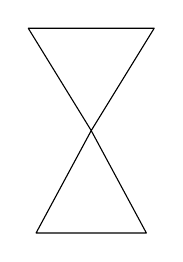
\begin{tikzpicture}[x=1mm,y=1mm,line cap=round,line join=round,font=\scriptsize]
\draw (64,-11) -- (80,-11) -- (72,-24) -- cycle;
\draw (72,-24) -- (65,-37) -- (79,-37) -- cycle;
\end{tikzpicture}
\end{document}
